\setcounter{table}{0}\setcounter{figure}{0}
\renewcommand{\thetable}{S3.\arabic{table}}
\renewcommand{\thefigure}{S3.\arabic{figure}}

\section*{Supplementary Material S3: Analyses and Comparators, Rounds 3--38}\label{sec:s3}

This section presents supporting tables and figures moved from the body of the manuscript so that the main text stays concise, covering hyperparameter details, the initial evaluation of the normative layer, comparators under equal treatment, leakage diagnosis analyses, external transfer, calibration, and clinical decision curves.

\subsection*{S3.1 Hyperparameters and computing environment}
\tabref{tab:hiper} lists the hyperparameters, hardware, and software.

{\scriptsize
\begin{longtable}{p{0.24\textwidth}p{0.70\textwidth}}
\caption{Hyperparameters and computing environment.}\label{tab:hiper}\\
\toprule
Component & Value \\
\midrule
\endfirsthead
\toprule
Component & Value \\
\midrule
\endhead
\bottomrule
\endfoot
Preprocessing & zero-phase FIR 0.5--45 Hz; 200 Hz; 10 s window; reject $>$800 $\mu$V \\
Logistic regression (I2, P3) & L2, lbfgs, balanced class weights, $C$ from 9 values $10^{-3}$--$10^{1}$, inner 5-fold CV (AUC) \\
P3 & 4th-order Butterworth; shrinkage $10^{-3}\,\mathrm{tr}/18$; a single global reference from training-patient windows; PCA 50 and adjustment on the components \\
NM & $d\in\{32,64\}$; $L\in\{32,96\}$ tokens; 2 BiMamba; AdamW $10^{-3}$, $10^{-2}$; batch 32; max. 60 epochs; 5 seeds \\
Rohira-log (round 36c) & Log band power $\ln x$ (values clipped at $10^{-12}$) per 10 s window; patient averaging (\textit{logpat}); \textit{random forest} with 100 trees \\
Tang symlog (round 37) & 506-dimensional per-second features; transform $\mathrm{symlog}(x) = \mathrm{sign}(x)\ln(1+|x|)$; 2 Bi-LSTM + attention \\
Hardware & Intel Core Ultra 9 285K; RAM 62 GB; NVIDIA RTX 4080 SUPER 16 GB \\
Software & Python 3.12.3; PyTorch 2.11.0; scikit-learn 1.9.1; NumPy 2.5.2; SciPy 1.18.1; MNE 1.13.2; pyriemann 0.12 \\
\end{longtable}
}

\subsection*{S3.2 Leakage test of the initial normative layer (V0) and sensitivity (V1--V4)}

{\scriptsize
\setlength{\tabcolsep}{3pt}
\begin{longtable}{p{0.36\textwidth}ccccc}
\caption{Hamdan-style \textit{confound} leakage test on the C1 and I2 pipelines without age and sex (50 canonical folds; 100 replicates per scenario). Pooled AUC in percent with the 5th--95th percentile across replicates; the last columns are the AUC within era strata as a validity diagnostic. Rule set beforehand: a mean I2 up to 52 means no evidence of leakage, 52--55 slight exploitation, and above 55 evidence of leakage.}\label{tab:hamdan}\\
\toprule
 & \multicolumn{2}{c}{Pooled AUC} & \multicolumn{2}{c}{Within-era AUC} \\
\cmidrule(lr){2-3}\cmidrule(lr){4-5}
Scenario & C1 & I2 & C1 & I2 \\
\midrule
\endfirsthead
\toprule
 & \multicolumn{2}{c}{Pooled AUC} & \multicolumn{2}{c}{Within-era AUC} \\
\cmidrule(lr){2-3}\cmidrule(lr){4-5}
Scenario & C1 & I2 & C1 & I2 \\
\midrule
\endhead
\bottomrule
\endfoot
H1: features shuffled across all patients & 50.8 [45.1--56.8] & 56.4 [51.1--62.4] & 50.7 & 51.4 \\
H2a: shuffled within era & 50.1 [44.2--57.2] & 55.8 [49.9--62.7] & 49.9 & 50.9 \\
H2b: shuffled within year $\times$ device & 47.1 [41.8--53.0] & 54.4 [47.6--60.3] & 47.7 & 48.7 \\
Real data (no shuffling) & 64.8 & 71.0 & 66.2 & 70.9 \\
\end{longtable}
}

\begin{table}[!htbp]
\caption{Sensitivity and leakage test of the normative layer on I2, P3, and NM (50 canonical folds). The H1 and H2a columns are the mean pooled AUC (percent) on uninformative features (without age and sex; I2 and P3: 100 replicates; NM: reduced version, 20 replicates, repetition 0 only, one configuration, H1 scenario). Rule set beforehand: up to 52 no leakage, 52--55 slight exploitation, above 55 leakage, and for NM additionally the 95th percentile of the mean up to 54. The next two columns are the per-fold AUC on real data without and with age and sex (Nadeau--Bengio 95\% CI). The AUC within year and device strata was computed for the variants with age and sex; the metadata baseline reached 43.2. The last column is the partial era test ($\eta^2$; $p$). V4 was added after the \textit{dry run} and before the full run; V0 is the same as I2; V4 and V5 (the counterpart of V4 for P3) are covariate regression on all training patients.}\label{tab:sensitivitas}\label{tab:kebocoran}
\centering\scriptsize
\setlength{\tabcolsep}{2pt}
\resizebox{\textwidth}{!}{%
\begin{tabular}{p{0.32\textwidth}cccccc}
\toprule
 & \multicolumn{2}{c}{Uninformative features} & \multicolumn{2}{c}{Real data: per-fold AUC} & Within strata & Partial era \\
\cmidrule(lr){2-3}\cmidrule(lr){4-5}
Variant & H1 & H2a & Without age/sex & With age/sex & year $\times$ device & $\eta^2$; $p$ \\
\midrule
C1 (no normative layer) & 50.6 & 51.6 & 65.6 [57.8--73.4] & 67.5 [59.0--76.0] & 72.9 & 0.03; 0.37 \\
I2--V0: current layer (training controls) & 56.0 & 57.1 & 71.7 [64.1--79.3] & 71.8 [63.8--79.9] & 75.1 & 0.11; 0.001 \\
I2--V1: separate reference (half of the training controls) & 56.1 & 56.3 & 67.0 [57.0--77.0] & 67.4 [58.1--76.8] & 73.9 & 0.14; 0.0002 \\
I2--V2: \textit{cross-fitted} & 55.7 & 56.8 & 71.4 [63.8--79.0] & 71.4 [63.6--79.2] & 74.8 & 0.10; 0.003 \\
I2--V3: no era & 52.5 & 53.7 & 66.4 [58.7--74.1] & 67.9 [59.8--76.1] & 73.6 & 0.02; 0.52 \\
I2--V4: covariate regression on all training patients (used) & 50.4 & 51.7 & 65.5 [56.8--74.2] & 68.0 [59.2--76.9] & 77.0 & 0.00; 0.98 \\
\midrule
P3: per-era alignment from training controls (old) & 55.5 & 55.6 & -- & -- & -- & -- \\
P3: per-era alignment from all training patients & 55.4 & 55.7 & -- & -- & -- & -- \\
P3--V5: global reference + covariate regression on PCA (used) & 49.8 & 50.0 & -- & -- & -- & -- \\
\midrule
NM: old normative layer (training controls) & 56.1 & -- & -- & -- & -- & -- \\
NM--V4: covariate regression on all training patients (used) & 51.5 & -- & -- & -- & -- & -- \\
\bottomrule
\end{tabular}
}
\end{table}

\subsection*{S3.3 Separate-track comparators and comparison with the literature}
\tabref{tab:pembanding} compares the comparators by track, and \tabref{tab:literatur} gives an indicative comparison with published studies.

{\scriptsize
\setlength{\tabcolsep}{3.2pt}
\begin{longtable}{p{0.28\textwidth}ccccccc}
\caption{Comparators under the same patient-level protocol (50 canonical folds), separated by track, with their own recipes (no covariate adjustment). AUC in percent; the 95\% CI of the per-fold AUC is Nadeau--Bengio corrected; metrics at the 0.5 threshold are descriptive. FT is \textit{fine-tuning} with official recipes without hyperparameter tuning; Tang-F uses 199 patients; frozen BENDR and LaBraM use embeddings with logistic regression; NA means not available.}\label{tab:pembanding}\\
\toprule
Model & Per-fold AUC [CI] & SD & Pooled AUC & Sens & Spec & BAC & Brier \\
\midrule
\endfirsthead
\toprule
Model & Per-fold AUC [CI] & SD & Pooled AUC & Sens & Spec & BAC & Brier \\
\midrule
\endhead
\bottomrule
\endfoot
\multicolumn{8}{l}{\textit{From-scratch track: reproduced published methods}} \\
Tang-F & 56.2 [47.7--64.7] & 8.2 & 54.9 & 51.6 & 55.1 & 53.4 & 0.267 \\
Rohira-F (channel set A) & 55.1 [46.5--63.8] & 8.3 & 55.0 & 55.3 & 47.4 & 51.4 & 0.260 \\
DNM-F & 61.8 [52.4--71.2] & 9.0 & 61.1 & 65.2 & 59.3 & 62.3 & 0.246 \\
\midrule
\multicolumn{8}{l}{\textit{\textit{Pretrained} track}} \\
Frozen BENDR & 55.5 [47.2--63.8] & 7.9 & 55.3 & 59.9 & 47.8 & 53.9 & 0.269 \\
Frozen LaBraM & 65.5 [57.7--73.4] & 7.5 & 64.0 & 60.3 & 59.5 & 59.9 & 0.237 \\
LaBraM-FT & 61.8 [54.0--69.6] & 7.5 & 61.0 & 55.7 & 57.7 & 56.7 & 0.296 \\
CBraMod-FT & 63.3 [54.8--71.7] & 8.1 & 62.6 & 50.9 & 66.2 & 58.6 & 0.285 \\
\end{longtable}
}

{\scriptsize
\setlength{\tabcolsep}{3pt}
\begin{longtable}{p{0.24\textwidth}p{0.18\textwidth}p{0.25\textwidth}p{0.13\textwidth}p{0.09\textwidth}}
\caption{Indicative comparison with published studies. Data, protocols, and metrics differ, so the figures are not directly comparable; the last three rows use the protocol of this study. RF is \textit{random forest}, PSD is \textit{power spectral density}, LOOCV is \textit{leave-one-out cross-validation}, and LOSO is \textit{leave-one-subject-out}.}\label{tab:literatur}\\
\toprule
Method [reference] & Data & Protocol & Metric & Result \\
\midrule
\endfirsthead
\toprule
Method [reference] & Data & Protocol & Metric & Result \\
\midrule
\endhead
\bottomrule
\endfoot
Rohira et al. \cite{rohira2023} (RF + PSD) & TUEP, 100/100 & Random 67/33 split; patient-level separation not stated & Accuracy & 95.73 \\
Tang et al. \cite{tang2024} & TUEP, 250 and 256 Hz & 5-fold; each segment tested once & Accuracy & 95.60 and 99.87 \\
Tang et al. \cite{tang2024} & TUEP, 86 patients with epilepsy & Per-subject LOOCV; patients with epilepsy only & Accuracy (= sensitivity) & 86.90 \\
Zanardini et al. \cite{zanardini2026} (\textit{preprint}) & TUEP subset, 31 subjects & LOSO; configuration selection without \textit{nested} & AUC & 97.3 $\pm$ 1.4 \\
Myers et al. \cite{myers2025} & 218 patients, 5 centers; initial EEG without abnormality & 10-fold CV (198 patients) & AUC & 0.940 $\pm$ 0.041 \\
Rohira-F (reproduction) & TUEP v2.0.1, 200 patients & Per patient, $10\times5$ folds & Pooled AUC & 55.0 \\
Tang-F (reproduction) & TUEP v2.0.1, 199 patients & Per patient, $10\times5$ folds & Pooled AUC & 54.9 \\
\textbf{F2 (this study)} & \textbf{TUEP v2.0.1, 200 patients} & \textbf{Per patient, first session, $10\times5$ folds} & \textbf{Per-fold (pooled) AUC} & \textbf{69.7 (69.4)} \\
\end{longtable}
}

\subsection*{S3.4 Comparators with equal treatment and tuning budget}
\tabref{tab:setara} gives the comparators under equal treatment, and \tabref{tab:anggaran} compares the default probe configuration with the one chosen by inner cross-validation.

{\scriptsize
\setlength{\tabcolsep}{3pt}
\begin{longtable}{p{0.30\textwidth}ccccc}
\caption{Per-fold AUC (percent) of comparators under equal treatment; all variants with age and sex were trained on the same folds. Covariate adjustment (V4) was fitted on all training patients; the BP row is C1 (without V4) and I2 (V4). The last column is the mean pooled AUC in the leakage test with shuffled features for the V4 variants (H1 / H2a; without age and sex; 20 replicates, except raw Rohira with 10 replicates; raw Tang-F repetition 0 only; Rohira log with 30 paired replicates). NA: not computed. $^\dagger$ The variant failed the absolute leakage test (AUC on uninformative features above 55); its AUC may contain adjustment-induced leakage. $^\ddagger$ Age and sex were added through logistic regression on the scores of the 32 validation patients of each fold. $^\mathsection$ Tang-Lp failed the paired rule R2 in scenario H1 ($\Delta = +3.7$ pp, one-sided 95\% upper bound $5.1 > 3.0$ pp).}\label{tab:setara}\\
\toprule
Comparator & None & + age/sex & V4 & V4 + age/sex & Null V4 \\
\midrule
\endfirsthead
\toprule
Comparator & None & + age/sex & V4 & V4 + age/sex & Null V4 \\
\midrule
\endhead
\bottomrule
\endfoot
Spectral BP (C1 / I2) & 65.6 & 67.5 & 65.5 & 68.0 & 50.4 / 51.7 \\
Frozen BENDR & 54.8 & 59.6 & 54.1 & 60.3 & 50.5 / 50.9 \\
Frozen LaBraM & 65.5 & 66.1 & 61.6 & 62.5 & 50.0 / 49.9 \\
DNM (57 metrics) & NA & 61.8 & NA & 53.9 & 50.0 / 51.4 \\
Raw Rohira (RF, window)$^\dagger$ & 55.1 & 60.9 & 56.7$^\dagger$ & 56.3$^\dagger$ & 57.3 / 56.2$^\dagger$ \\
Rohira log (RF, \textit{logpat}) & 55.1 & 60.9 & 54.7 & 60.8 & 50.7 / 51.8 \\
Raw Tang-F (Bi-LSTM)$^\dagger$ & 56.2 & 58.9$^\ddagger$ & 61.7$^\dagger$ & 60.3$^\dagger$$^\ddagger$ & 60.5 / 59.6$^\dagger$ \\
Tang symlog (Bi-LSTM, \textit{Lp})$^\mathsection$ & 60.8 & 62.1 & 59.0$^\mathsection$ & 59.8$^\mathsection$ & 51.5 / 52.2$^\mathsection$ \\
\end{longtable}
}

{\scriptsize
\setlength{\tabcolsep}{4pt}
\begin{longtable}{p{0.34\textwidth}cccc}
\caption{Per-fold AUC (percent) with the default probe configuration (L2 logistic regression) and with the configuration chosen by inner cross-validation in the same search space for all pipelines (six configurations); all variants use age and sex. V4 adjustment and PCA were refitted in every inner fold.}\label{tab:anggaran}\\
\toprule
 & \multicolumn{2}{c}{No adjustment} & \multicolumn{2}{c}{V4 adjustment} \\
\cmidrule(lr){2-3}\cmidrule(lr){4-5}
Pipeline & Default & Tuned & Default & Tuned \\
\midrule
\endfirsthead
\toprule
 & \multicolumn{2}{c}{No adjustment} & \multicolumn{2}{c}{V4 adjustment} \\
\cmidrule(lr){2-3}\cmidrule(lr){4-5}
Pipeline & Default & Tuned & Default & Tuned \\
\midrule
\endhead
\bottomrule
\endfoot
Spectral BP (C1 / I2) & 67.5 & 66.1 & 68.0 & 65.8 \\
Frozen BENDR & 59.6 & 59.3 & 60.3 & 58.9 \\
Frozen LaBraM & 66.1 & 66.5 & 62.5 & 65.6 \\
DNM & 61.8 & 60.1 & 53.9 & 54.1 \\
\end{longtable}
}\clearpage

\subsection*{S3.5 Diagnosis of the leakage mechanism and feature distribution}
\tabref{tab:diagnosis} gives the factorial diagnosis of the leakage mechanism, \tabref{tab:kurtosis} the skewness and kurtosis of the features, and \tabref{tab:paired} the paired permutation test against the baseline without covariate adjustment.

\begin{table}[!htbp]
\caption{Factorial diagnosis of the leakage mechanism on the Rohira representation (50 canonical folds). Each cell holds the mean pooled AUC over 10 replicates of the leakage test (except the paired control $n=30$). Scenario H1 moves the whole EEG block of each patient (all windows and features) to another patient by one permutation of all patients; H2a does the same within recording era; labels and covariates stay with the patient (\tabref{tab:definisi_null} of the main text). The \textit{win} variant fits adjustment per window; \textit{pat} fits adjustment on the per-patient feature mean; \textit{cross-fit} (\textit{win\_x}, \textit{pat\_x}) fits the coefficients of each training patient on the other training patients (five groups); log applies $\ln x$ before adjustment.}\label{tab:diagnosis}
\centering\scriptsize
\setlength{\tabcolsep}{2.5pt}
\resizebox{\textwidth}{!}{%
\begin{tabular}{p{0.22\textwidth}p{0.16\textwidth}p{0.24\textwidth}ccc}
\toprule
Classifier & Feature scale & Adjustment variant & H1 & H2a & Remark \\
\midrule
\textit{Random forest} & Raw & No adjustment ($n=30$) & 50.1 & 52.0 & Paired control \\
\textit{Random forest} & Raw & Per window (\textit{win}, V4) & 57.3 & 56.2 & Leaks \\
\textit{Random forest} & Raw & Patient mean (\textit{pat}) & 57.5 & 56.3 & Leaks ($H_A$ rejected) \\
\textit{Random forest} & Raw & Window \textit{cross-fit} (\textit{win\_x}) & 56.6 & 56.2 & Leaks ($H_B$ rejected) \\
\textit{Random forest} & Raw & Patient \textit{cross-fit} (\textit{pat\_x}) & 56.4 & 56.3 & Leaks ($H_B$ rejected) \\
Logistic regression & Raw & No adjustment & 48.4 & 52.5 & No evidence of leakage \\
Logistic regression & Raw & Per window (\textit{win}) & 52.4 & 51.5 & No evidence of leakage \\
Logistic regression & Raw & Patient mean (\textit{pat}) & 50.8 & 51.3 & No evidence of leakage \\
\textit{Random forest} & Log $\ln x$ & Per window (\textit{logwin}, 10 rep) & 53.0 & 53.7 & Suppressed ($H_C$ supported) \\
\textit{Random forest} & Log $\ln x$ & Patient mean (\textit{logpat}, 10 rep) & 52.3 & 53.8 & Suppressed ($H_C$ supported) \\
\textit{Random forest} & Log $\ln x$ & Patient mean (\textit{logpat}, $n=30$) & 50.7 & 51.8 & No evidence of leakage (R1 and R2) \\
\bottomrule
\end{tabular}
}
\end{table}

\begin{table}[!htbp]
\caption{Skewness and kurtosis of the raw and transformed features (before covariate adjustment), computed per feature in double precision over all observation units of each representation. Kurtosis is Fisher excess kurtosis ($0$ for a normal distribution); the columns give the median and the maximum over features, and the last column the largest absolute feature value. Each reproduced method used its own segmentation: Rohira 10 s windows over the whole recording without artifact rejection (28,982 windows; the main pipeline has 27,596 windows before and 26,968 after rejection), Tang 4,702 sequences of 60 one-second steps from 199 patients (282,120 seconds), and NM 4 s segments (66,106). Symlog is $\mathrm{sign}(x)\ln(1+|x|)$; the Rohira log pipeline used $\ln x$. The values were recomputed by script in round 49; the earlier version of this table reported the largest absolute Tang value ($8\times10^{8}$) as a kurtosis and computed the Tang and NM rows on subsamples.}\label{tab:kurtosis}
\centering\scriptsize
\setlength{\tabcolsep}{2.5pt}
\resizebox{\textwidth}{!}{%
\begin{tabular}{p{0.22\textwidth}p{0.10\textwidth}p{0.20\textwidth}ccccc}
\toprule
Feature & Scale & Observation unit ($n$) & Features & Median kurtosis & Maximum kurtosis & Median skewness & Max.\ $|x|$ \\
\midrule
Rohira (band power) & Raw & Windows (28,982) & 48 & 8,481 & 20,816 & +84.70 & $1.4\times10^{7}$ \\
Rohira (band power) & Raw & Patient mean (200) & 48 & 110 & 189.1 & +10.25 & $2.1\times10^{5}$ \\
Rohira (band power) & $\ln x$ & Windows (28,982) & 48 & 2.96 & 5.07 & $-$0.32 & 16.4 \\
Rohira (band power) & $\ln x$ & Patient mean (200) & 48 & 2.06 & 5.26 & $-$0.49 & 10.3 \\
Tang-F (spatial projection) & Raw & Seconds (282,120) & 506 & 28,394 & 225,407 & +1.05 & $8.3\times10^{8}$ \\
Tang-F (spatial projection) & Symlog & Seconds (282,120) & 506 & $-$1.56 & 0.79 & $-$0.03 & 20.5 \\
NM (temporal representation) & Raw & Segments (66,106) & 114 & 0.87 & 8.29 & $-$0.79 & 12.2 \\
\bottomrule
\end{tabular}
}
\end{table}

\begin{table}[!htbp]
\caption{Paired permutation leakage test against the baseline without covariate adjustment on 50 canonical folds. Scenario H1 moves whole patient EEG blocks between all patients and H2a within recording era, with labels and covariates kept (\tabref{tab:definisi_null} of the main text). $n$ is the number of random replicates. The columns give the mean AUC without adjustment, the AUC with adjustment (percent), the paired difference $\Delta$ in pp (standard error, SE), the one-sided 95\% upper bound ($\Delta + 1.645\,\mathrm{SE}$), the $p$ value of the paired one-sample $t$-test, the decision of rule R2 set in the plan, and the one-sided 95\% upper bound of rule R1.}\label{tab:paired}
\centering\scriptsize
\setlength{\tabcolsep}{1.4pt}
\resizebox{\textwidth}{!}{%
\begin{tabular}{p{0.18\textwidth}cccccccc}
\toprule
Model & Scenario & Control AUC & Test AUC & $\Delta$ (SE) & $\Delta_{95}$ & $p$ & R2 decision & R1 bound \\
\midrule
Rohira-logpat ($n=30$) & H1 & 50.1 & 50.7 & $+0.6$ (0.5) & $+1.3$ & 0.253 & no evidence of leakage & 52.1 \\
Rohira-logpat ($n=30$) & H2a & 52.0 & 51.8 & $-0.3$ (0.3) & $+0.3$ & 0.454 & no evidence of leakage & -- \\
Tang-Lp ($n=20$) & H1 & 47.7 & 51.5 & $+3.7$ (0.8) & $+5.1$ & <0.001 & leakage & 52.7 \\
Tang-Lp ($n=20$) & H2a & 49.4 & 52.2 & $+2.8$ (0.7) & $+4.0$ & 0.0010 & slight exploitation/uncertain & -- \\
NM-V4 ($n=20$) & H1 & 49.0 & 51.5 & $+2.6$ (0.8) & $+3.9$ & 0.005 & slight exploitation/uncertain & 53.1 \\
NM-V4 ($n=20$) & H2a & 51.3 & 50.6 & $-0.7$ (0.9) & $+0.7$ & 0.436 & no evidence of leakage & -- \\
\bottomrule
\end{tabular}
}
\end{table}

\subsection*{S3.6 Confounder test, calibration, decision curves, and external transfer}
\tabref{tab:confounder} gives the confounder test, \figref{fig:kalibrasi} the calibration of F2 and I2, and \figref{fig:keputusan} the decision curves.

\begin{table}[!htbp]
\caption{Spis\'ak-style \textit{confounder} test on \textit{out-of-fold} scores averaged over 10 repetitions. Each cell holds $\eta^2$ (or $r^2$ for age) and the $p$ value of the conditional permutation test with 10,000 permutations; for F2 and NM on era, $p$ is $p_{\mathrm{Holm}}$ within the primary family (two partial tests), otherwise the raw $p$. The smallest resolution of $p$ is 0.0001.}\label{tab:confounder}
\centering\scriptsize
\setlength{\tabcolsep}{1.5pt}
\resizebox{\textwidth}{!}{%
\begin{tabular}{p{0.20\textwidth}ccccccc}
\toprule
 & \multicolumn{4}{c}{Partial test: $\eta^2$; $p$} & \multicolumn{3}{c}{Full test: $p$} \\
\cmidrule(lr){2-5}\cmidrule(lr){6-8}
Model & Era & Device & Montage & Age & Era & Device & Year $\times$ device \\
\midrule
F2 & 0.01; 1.00 & 0.00; 0.87 & 0.00; 0.71 & 0.13; $\leq$0.0001 & $\leq$0.0001 & $\leq$0.0001 & $\leq$0.0001 \\
I2 & 0.00; 0.98 & 0.00; 0.87 & 0.00; 0.75 & 0.17; $\leq$0.0001 & $\leq$0.0001 & $\leq$0.0001 & $\leq$0.0001 \\
P3 & 0.02; 0.54 & 0.01; 0.51 & 0.01; 0.12 & 0.13; $\leq$0.0001 & $\leq$0.0001 & $\leq$0.0001 & $\leq$0.0001 \\
NM & 0.02; 1.00 & 0.01; 0.73 & 0.00; 0.60 & 0.05; 0.013 & $\leq$0.0001 & $\leq$0.0001 & $\leq$0.0001 \\
C1 (no adjustment) & 0.03; 0.37 & 0.00; 0.92 & 0.00; 0.47 & 0.14; $\leq$0.0001 & $\leq$0.0001 & $\leq$0.0001 & $\leq$0.0001 \\
Metadata baseline & 0.46; $\leq$0.0001 & 0.36; $\leq$0.0001 & 0.10; $\leq$0.0001 & 0.01; 0.44 & 0.049 & 0.003 & 0.82 \\
F2 with the old normative layer & 0.17; $\leq$0.0001 & 0.03; 0.13 & 0.05; 0.001 & 0.16; $\leq$0.0001 & $\leq$0.0001 & $\leq$0.0001 & $\leq$0.0001 \\
LaBraM-FT & 0.02; 0.64 & 0.01; 0.59 & 0.00; 0.88 & 0.04; 0.016 & 0.0002 & 0.0003 & 0.0004 \\
CBraMod-FT & 0.03; 0.40 & 0.01; 0.61 & 0.00; 0.81 & 0.05; 0.008 & $\leq$0.0001 & $\leq$0.0001 & $\leq$0.0001 \\
\bottomrule
\end{tabular}
}
\end{table}

\begin{figure}[!htbp]
\centering
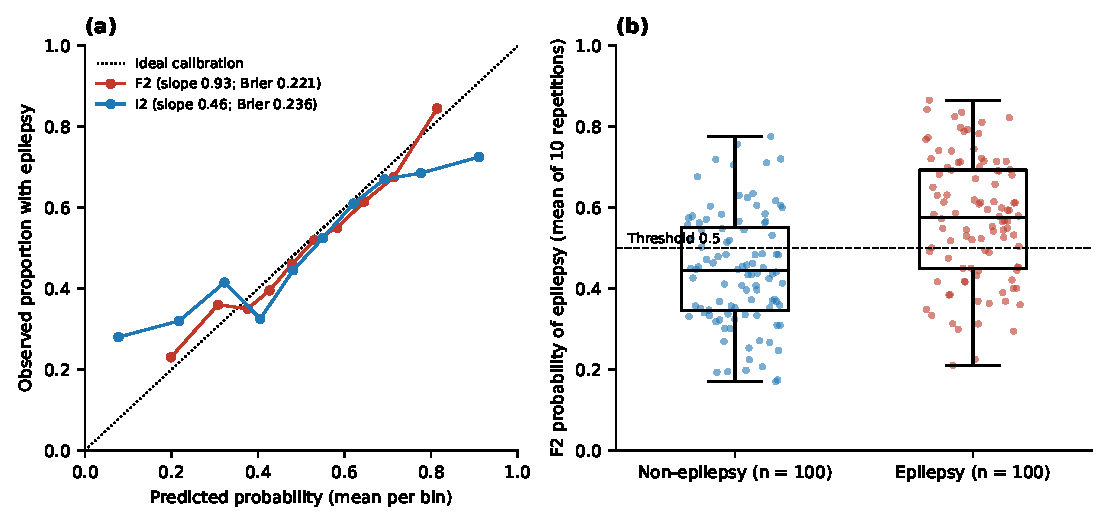
\includegraphics[width=0.85\textwidth]{figures_en/hasil_kalibrasi_pasien.pdf}
\caption{(a) Reliability diagram of F2 and I2 from \textit{out-of-fold} predictions (10 quantile bins over 2,000 predictions from 10 repetitions). (b) F2 probability of epilepsy averaged over 10 repetitions for each patient, by class; boxes show the median and quartiles and the dashed line marks the 0.5 threshold.}\label{fig:kalibrasi}
\end{figure}

\begin{figure}[!htbp]
\centering
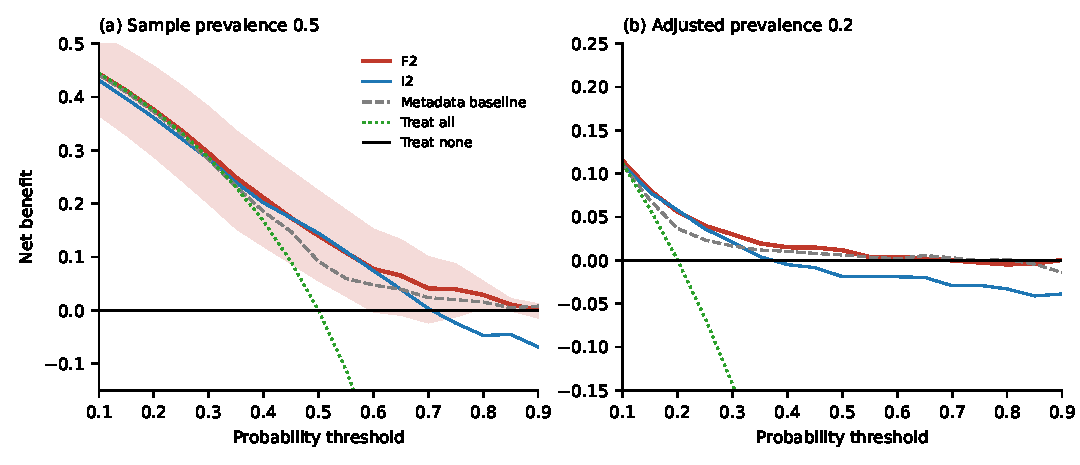
\includegraphics[width=0.85\textwidth]{figures_en/hasil_kurva_keputusan.pdf}
\caption{Decision curves (\textit{net benefit}) from \textit{out-of-fold} predictions averaged over 10 repetitions. (a) Sample prevalence 0.5; the band shows the patient-\textit{bootstrap} 95\% CI for F2 (2,000 replicates). (b) Adjusted prevalence 0.2, assuming scores calibrated at a prevalence of 0.5; no CI and descriptive only.}\label{fig:keputusan}
\end{figure}

\subsubsection*{Details of external transfer, feature stability, and error analysis}
In the Kural cohort (99 subjects; short sharp-wave segments), the frozen TUEP model gave an AUC of 62.2 for C1 (\textit{bootstrap} 95\% CI 50.7--73.0; $p_{\mathrm{Holm}} = 0.100$ vs 50) and 57.1 for I2 with covariate adjustment (44.9--68.2; $p = 0.23$ vs 50). The difference of I2 against C1 was $-5.1$ pp (CI $-10.9$ to $-0.6$; $p = 0.028$). The Kural demographic baseline reached 63.4 (95\% CI 52.7--73.8; computed afterwards, S2.16). Of the 313 Emotiv subjects, 290 had a clean eyes-closed window and contributed to the transfer (the other 23 had no window that passed the label-free artifact thresholds). With frozen TUEP preprocessing statistics, transfer from TUEP to Emotiv gave an AUC of 56.5 (49.8--63.0); after standardizing each cohort with its own unlabeled features (transductive adaptation), it gave 54.1 (47.2--60.7), and the reverse transfer 54.8 (47.0--62.5) and 54.0 (45.8--61.9).
The I2 deviation pattern is not focal: total power was higher in the epilepsy group (mean $d$ $+0.35$; CI excluded 0 in 17 of 19 channels). By contrast, the relative bands were small ($d$ $+0.06$ delta, $+0.07$ theta, $+0.04$ alpha, $+0.02$ beta, $-0.18$ gamma; 0 of 19 channels).
In 108 patients with later sessions, I2 reached a pooled AUC of 66.5 on the later session and 68.8 on the first session (Spearman 0.74). A total of 28 patients (14\%; 16 with epilepsy, 12 without) were misclassified consistently; hard-to-classify patients without epilepsy had a median age of 44.5 versus 63 years ($q = 0.004$).
